\documentclass[12pt]{article}
\usepackage[utf8]{inputenc}
\usepackage[hidelinks]{hyperref}
\usepackage[a4paper]{geometry}
\usepackage{amssymb}
\usepackage{graphicx}
\usepackage{fancyhdr}
\usepackage{floatrow}
\graphicspath{{./}}
\usepackage{booktabs,makecell}
\usepackage{titlesec}

\titleformat*{\section}{\LARGE\bfseries}
\titleformat*{\subsection}{\Large\bfseries}

\pagestyle{fancy}

\lhead{\leftmark}
\rhead{Page \thepage}
\cfoot{Chebyschev Bandpass Filter}
\renewcommand{\footrulewidth}{1pt}

\begin{document}

\begin{titlepage}
\begin{center}
    \vspace*{\fill}
\includegraphics[scale=0.6]{iitb_logo.jpg}\\
[4 cm]
    \rule{12.5cm}{0.75mm}\\
    \huge{\bfseries Filter Design Assignment-II}
    \rule{12.5cm}{0.75mm}\\
    [0.5cm]
   {\textbf {EE338 - 2023 \\
    Chebyschev Bandpass Filter Review Report}}\\
    [2cm]
\end{center}
\begin{flushleft}
   {\huge
    Name:- Omkar Nitsure \\
    Roll Number:- 210070057 \\
     \\}
    \end{flushleft}
\end{titlepage}
\tableofcontents

\pagestyle{fancy}

\fancyhead{}
\fancyhead[L]{\textbf{Filter Design(Chebyschev Bandpass)}}
\fancyhead[R]{\textbf{Omkar Nitsure(210070057)}}
\fancyfoot{}
\fancyfoot[C]{\thepage}
\newpage
\section{Student Details:-}
\textbf{Name}:- Omkar Nitsure\\
\textbf{Roll no}:- 210070057\\
\textbf{Filter Number}:- 107\\

\section{Chebyschev Bandpass Filter}
\subsection{Discrete Time Filter Specifications}

Filter Number Assigned = \textbf{107}\\
As Filter number $>$ 80, we get the modified $\textbf{m} = 107 - 80 = \textbf{27}$\\
$q(m) =$ greatest integer strictly less than 0.1m
Thus for $m = 27$, we get $\textbf{q(m) = 2}$\\
$\textbf{r(m)} = m - 10q(m) = 27 - 10(2) = \textbf{7}$\\
$\textbf{BL(m)} = 10 + 5q(m) + 13r(m) = 10 + 5(2) + 13(7) = \textbf{111}$\\
$\textbf{BH(m)} = BL(m) + 75 = 111 + 75 = \textbf{186}$\\
\par

As the Sampling Frequency is more than \textbf{Twice} the maximum frequency in the signal, there will be no Aliasing according to \textbf{Nyquist Theorem.}
\noindent So the Specifications of the \textbf{Bandpass Filter} to be designed are as follows:-

\begin{itemize}
    \item \textbf{Sampling Frequency} = 600 kHz
    \item \textbf{Passband} = 111 kHz to 186 kHz
    \item \textbf{Transition band} = 5 kHz on either side of passband
    \item \textbf{Stopband} = 0-106 kHz and 191-300 kHz
    \item \textbf{Tolerance} = 0.15 for both passband and stopband
    \item \textbf{Passband Nature} = Equiripple
    \item \textbf{Stopband Nature} = Monotonic
\end{itemize}
\newpage

\subsection{Normalized Digital Filter Specifications}
The above frequency response can be normalized in a range of $-\pi$ to $-\pi$ by normalization where the Sampling frequency maps to 2$\pi$ on the normalized frequency axis and the other frequencies map accordingly.\\
\textbf{Sampling Frequency = $\Omega_{s}$ = 600 kHz}

\[\omega = \frac{2\pi*\Omega}{\Omega_{s}}\]

Thus the corresponding normalized discrete filter specifications are:-
\begin{itemize}
    \item \textbf{Passband} = 0.37$\pi$ to 0.62$\pi$
    \item \textbf{Transition Band} = 0.0167$\pi$ on either side of passband
    \item \textbf{Stopband} = 0-0.3533$\pi$ and 0.6367$\pi$-$\pi$
    \item\textbf{Tolerance} = 0.15 in magnitude for both passband and stopband
    \item \textbf{Passband Nature} = Equiripple
    \item \textbf{Stopband Nature} = Monotonic
\end{itemize}

\subsection{Bandpass Analog Filter Specifications using Bilinear Transformation}
The Digital to Analog domain bilinear transformation is as follows:-

\[\Omega = tan(\frac{\omega}{2})\]

\noindent
We will now use this bilinear transformation to get the corresponding frequencies in the Analog domain for the above frequencies in the digital domain.

\begin{center}
    \begin{tabular}{|c|c|}
     \hline
    $\omega$ & $\Omega$ \\ \hline
    0.37$\pi$ & 0.6569 \\ \hline
    0.62$\pi$ & 1.4714 \\ \hline
    0.3533$\pi$ & 0.62 \\ \hline
    0.6367$\pi$ & 1.5577 \\ \hline
    0 & 0 \\ \hline
    $\pi$ & $\infty$ \\ \hline
    \end{tabular}
\end{center}
\newpage

\noindent

Thus the specifications of the corresponding Analog filter of the same type are as follows:-

\begin{itemize}
    \item \textbf{Passbandband} = 0.6569 ($\Omega_{p1}$) to 1.4714 ($\Omega_{p2}$)
    \item \textbf{Transition Band} = 0.62 to 0.6569 and 1.4714 to 1.5577
    \item \textbf{Stopband} = 0 to 0.0.62($\Omega_{s1}$) and 1.5577($\Omega_{s2}$) to $\infty$
    \item\textbf{Tolerance} = 0.15 in magnitude for both passband and stopband
    \item \textbf{Passband Nature} = Equiripple
    \item \textbf{Stopband Nature} = Monotonic
\end{itemize}

\subsection{Frequency Transformation to Analog Lowpass Filter Specifications}

Now, that we have the specifications of the corresponding Analog Filter, we can use the frequency transformation to get the specifications of the corresponding Analog Lowpass filter which can then be designed in practice easily. The transformation we choose to use is given as follows:-

\[\Omega_{L} = \frac{\Omega^2 - \Omega_{0}^2}{B\Omega}\]

While calculating the 2 parameters \textbf{B} and \textbf{$\Omega_{0}$}, we choose to transform the passband edges namely $\Omega_{p1}$ and $\Omega_{p2}$ to -1 and 1. Other frequencies then get mapped accordingly.

\[\Omega_{0} = \sqrt{\Omega_{p1}\Omega_{p2}} = \sqrt{0.6569*1.4714} = 0.98314\]

\[B = \Omega_{p2} - \Omega_{p1} = 1.4714 - 0.6569 = 0.8146\]

\begin{center}
    \begin{tabular}{|c|c|}
     \hline
    $\Omega$ & $\Omega_{L}$ \\ \hline
    $0^+$ & $-\infty$ \\ \hline
    0.6569 ($\Omega_{P1}$) & -1 ($\Omega_{LP1}$)\\ \hline
    1.4714 ($\Omega_{P2}$) & +1 ($\Omega_{LP2}$)\\ \hline
    0.98314 ($\Omega_{0}$) & 0 \\ \hline
    0.62 ($\Omega_{S1}$) & -1.1526 ($\Omega_{LS1}$) \\ \hline
    1.5577 ($\Omega_{S2}$) & 1.1504 ($\Omega_{LS2}$) \\ \hline
    $\infty$ & $\infty$ \\ \hline
    \end{tabular}
\end{center}

\subsection{Frequency Transformed Lowpass Analog Filter Specifications}

\begin{itemize}
    \item \textbf{Passband Edge} = 1 ($\Omega_{LP}$)
    \item \textbf{Stopband Edge}= min(-$\Omega_{LS1}$,$\Omega_{LS2}$)= min(1.1526,1.1504) = 1.1504 ($\Omega_{LS}$)
    \item\textbf{Tolerance} = 0.15 in magnitude for both passband and stopband
    \item \textbf{Passband Nature} = Equiripple
    \item \textbf{Stopband Nature} = Monotonic
\end{itemize}

\subsection{Lowpass Analog Filter Transfer Function}
Now, that we have transformed the initial Digital Filter Specifications to the corresponding Analog Lowpass Filter specifications, we are ready to design the Analog Lowpass Filter using the \textbf{Chebyschev} approximation. We need the following quantities for that purpose:-\\
The tolerance for both Stopband and Passband is \textbf{$\delta$ = 0.15}

\[D_{1} = \frac{1}{(1 - \delta)^2} - 1 = \frac{1}{0.85^2} - 1 = 0.3841\]

\[D_{2} = \frac{1}{\delta^2} - 1 = \frac{1}{0.15^2} - 1 = 43.44\]

Now we find out the \textbf{Order of the Chebyschev Filter(N)} using the following formula where we choose the parameter $\epsilon$ of the \textbf{Chebyschev Filter} to be $\sqrt{D_{1}}$:-

\[N_{min} = \lceil \frac{cosh^{-1}(\sqrt{\frac{D2}{D1}})}{cosh^{-1}(\frac{\Omega_{S}}{\Omega_{P}})} \rceil = \lceil 5.6378 \rceil = 6\]

Now we can directly solve for the poles of the Transfer Function of the Analog Lowpass Filter using the following Equation:-

\[1 + D_{1}cosh^{2}(N_{min}cosh^{-1}(\frac{s}{j})) = 1 + 0.3841cosh^{2}(6cosh^{-1}(\frac{s}{j})) = 0\]

Solving this equation in WolframAlpha, we get the following 6 roots in the Left half of the Complex s plane (The reason for choosing only the left half plane poles is that they are stable):-
\[p_{1} = -0.05458 + 0.98717j\]
\[p_{2} = -0.05458 - 0.98717j\]
\[p_{3} = -0.2037 + 0.26451j\]
\[p_{4} = -0.2037 - 0.26451j\]
\[p_{5} = -0.14912 + 0.72266j\]
\[p_{6} = -0.14912 + 0.72266j\]

The plot of the poles of the magnitude response of the Analog Lowpass Filter plotted using python after Solving the Equation is as follows:-

\begin{figure}[H]
    \centering
    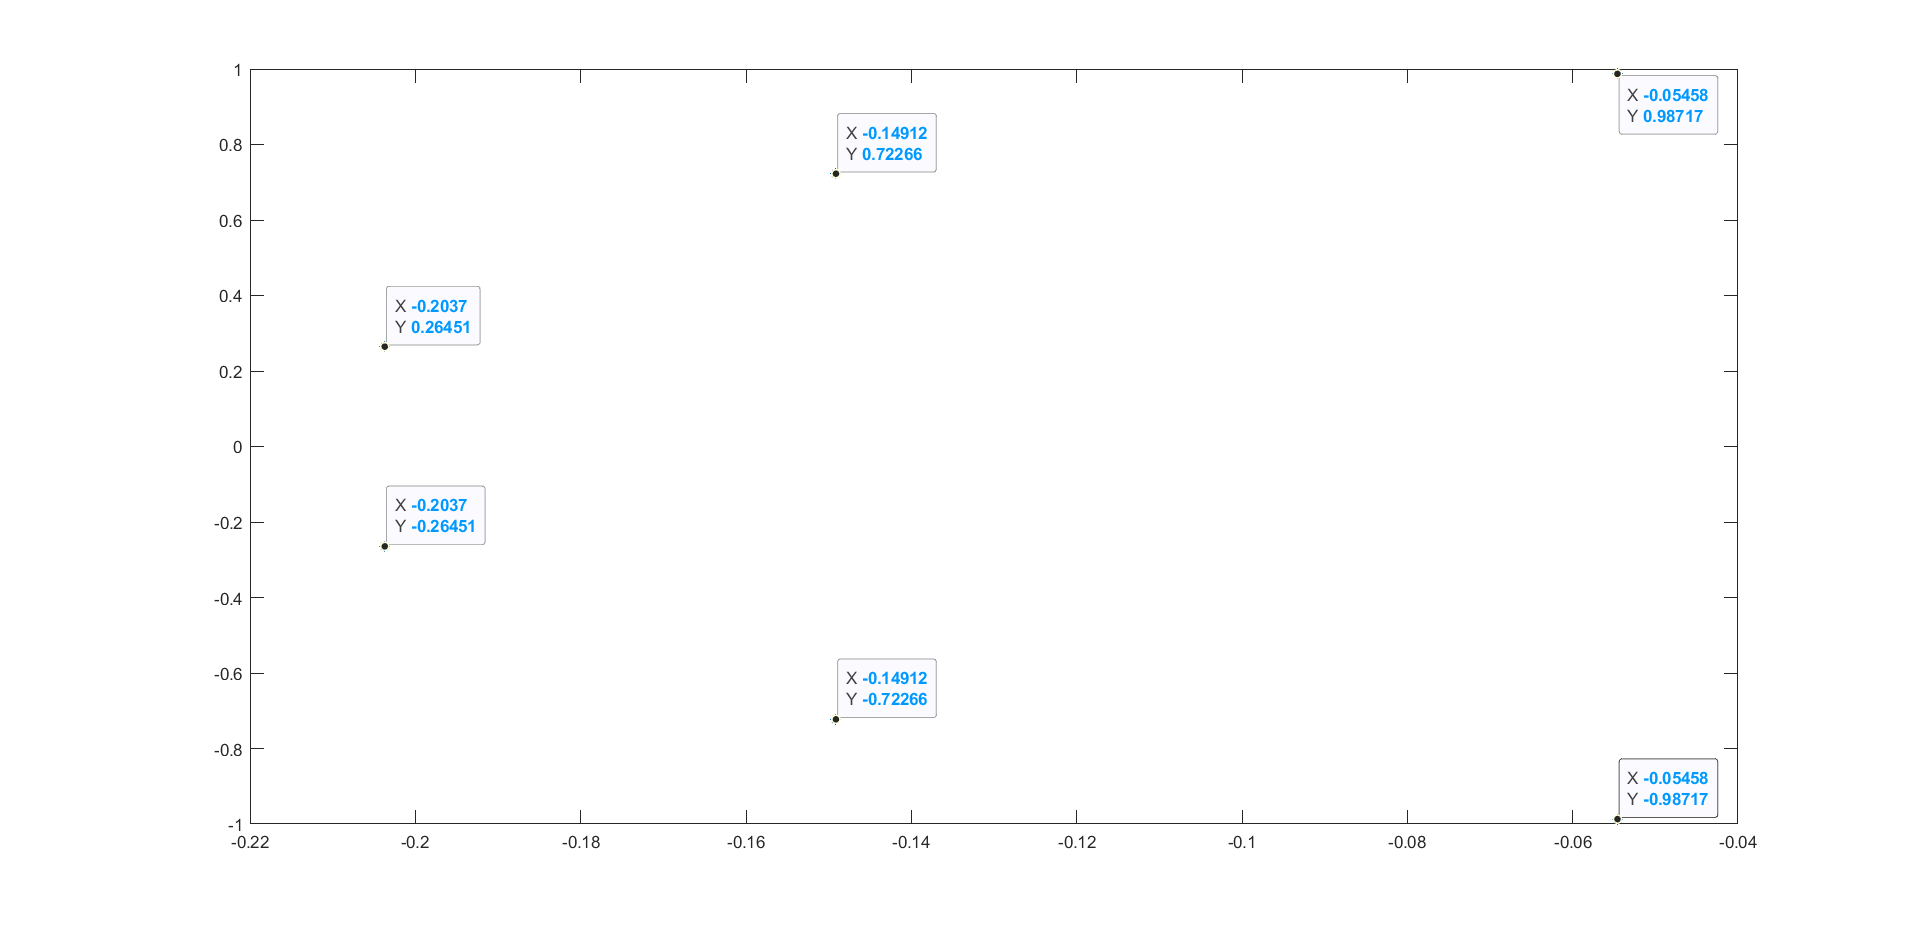
\includegraphics[width =\textwidth, height=8cm]{poles.png}
    \caption{Poles of Magnitude response of Analog Lowpass Filter}
\end{figure}

As now we have the poles, we can finally write down the Transfer Function of the Analog Lowpass Filter. We make use of the fact that \textbf{N} is \textbf{even} to find the DC gain of the filter. As \textbf{N} is even we know that the DC gain is $\frac{1}{\sqrt{1+\epsilon^{2}}}$. We also use the fact that we have used $\epsilon = \sqrt{D_{1}}$

\[H_{analog,LPF}(s_{L}) = \frac{(-1)^{6}p_{1}p_{2}p_{3}p_{4}p_{5}p_{6}}{\sqrt{1+D_{1}}(s_{L} - p_{1})(s_{L} - p_{2})(s_{L} - p_{3})(s_{L} - p_{4})(s_{L} - p_{5})(s_{L} - p_{6})}\]

\[\scalebox{1.1}{$H_{analog,LPF}(s_{L}) = \frac{0.050422}{(s_{L}^2+0.10916s_{L}+0.97748)(s_{L}^2+0.4074s_{L}+0.11146)(s_{L}^2+0.29824s_{L}+0.54447)}$}\]

\subsection{Analog Bandpass Transfer Function}

Now we need to transform the Analog Lowpass Filter back to the Analog Bandpass Filter using the same transformation we used earlier.
\[s_{L} = \frac{\Omega_{0}^2 + s^2}{Bs}\]
Thus
\[s_{L} = \frac{0.96656 + s^2}{0.81458s}\]

Substituting this value of $s_{L}$ into the above Analog Lowpass Filter Tranfer Function, we get the Analog Bandpass Filter Transfer function i.e \textbf{$H_{analog,BPF}(s)$}. As it is a Rational Transfer function, we can write \textbf{2 series} in Numerator and Denominator where the coefficients of different degrees of \textbf{s} are as follows:-

\begin{table}[H]
  \begin{minipage}{.5\linewidth}
    \centering
    \begin{tabular}{ |c|c| }
      \toprule
      \makecell{Powers of s \\ in Denominator} & \makecell{Coefficients} \\
      \midrule
      $s^{12}$ & 1 \\
      $s^{11}$ & 0.6637 \\
      $s^{10}$ & 7.015 \\
      $s^{9}$ & 3.7642 \\
      $s^{8}$ & 19.087 \\
      $s^{7}$ & 7.9064 \\
      $s^{6}$ & 25.6136 \\
      $s^{5}$ & 7.6420 \\
      $s^{4}$ & 17.832 \\
      $s^{3}$ & 3.3991 \\
      $s^{2}$ & 6.1228 \\
      $s^{1}$ & 0.5599 \\
      $s^{0}$ & 0.8154 \\
      \bottomrule
    \end{tabular}
  \end{minipage}%
  \begin{minipage}{.5\linewidth}
    \centering
    \begin{tabular}{ |c|c| }
      \toprule
      \makecell{Powers of s \\ in Numerator} & \makecell{Coefficients} \\
      \midrule
      $s^{6}$ & 0.0147 \\
      \bottomrule
    \end{tabular}
  \end{minipage}
\end{table}

\newpage

\subsection{Discrete Time Filter Transfer Function}
Finally, to transform the Analog Bandpass Transfer Function into the Discrete Bandpass Transfer Function with \textbf{Chebyschev} Approximation, we need to make use of the Bilinear Transformation which is given as:-
\[s = \frac{1 - z^{-1}}{1 + z^{-1}}\]

Substituting the above equation in the Analog Bandspass Filter Transfer Function we get $H_{Digital,BPF}(z)$. It can be written in the form
N(z)/D(z) where the coefficients of the polynomials N(z) and D(z) are given as follows:-

\begin{table}[H]
  \begin{minipage}{.5\linewidth}
    \centering
    \begin{tabular}{ |c|c| }
      \toprule
      \makecell{Powers of $z^{-1}$ \\ in Numerator} & \makecell{Coefficients} \\
      \midrule
      $z^{-12}$ & 0.528 \\
      $z^{-11}$ & -0.1047 \\
      $z^{-10}$ & 2.9969 \\
      $z^{-9}$ & -0.51 \\
      $z^{-8}$ & 7.5532 \\
      $z^{-7}$ & -1.0604 \\
      $z^{-6}$ & 10.7999 \\
      $z^{-5}$ & -1.1757 \\
      $z^{-4}$ & 9.2537 \\
      $z^{-3}$ & -0.6974 \\
      $z^{-2}$ & 4.5273 \\
      $z^{-1}$ & -0.1788 \\
      $z^{0}$ & 1 \\
      \bottomrule
    \end{tabular}
  \end{minipage}%
  \begin{minipage}{.5\linewidth}
    \centering
    \begin{tabular}{ |c|c| }
      \toprule
      \makecell{Powers of $z^{-1}$ \\ in Denominator} & \makecell{Coefficients} \\
      \midrule
      $z^{-12}$ & 0.000145 \\
      $z^{-10}$ & -0.00087 \\
      $z^{-8}$ & 0.00218 \\
      $z^{-6}$ & -0.002905 \\
      $z^{-4}$ & 0.00218 \\
      $z^{-2}$ & -0.00087 \\
      $z^{0}$ & 0.000145 \\
      \bottomrule
    \end{tabular}
  \end{minipage}
\end{table}

\subsection{ Plots of Magnitude Response and Phase Response of the Chebyschev Bandpass Filter}

\begin{figure}[H]
    \centering
    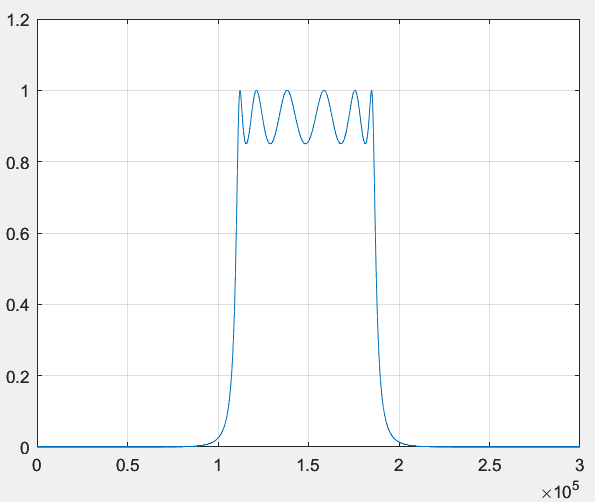
\includegraphics[width =\textwidth, height=8cm]{magnitude_response_chebyschev.png}
    \caption{Magntitude Response of the Filter in Frequency}
\end{figure}

\begin{figure}[H]
    \centering
    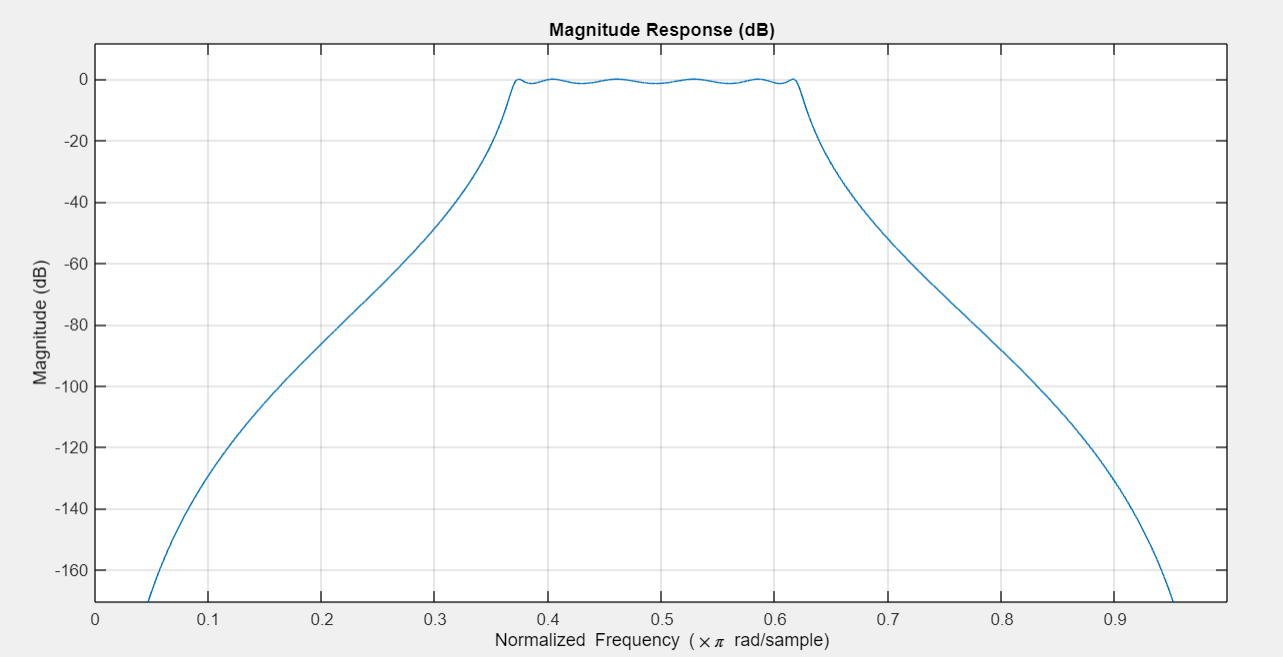
\includegraphics[width =\textwidth, height=8cm]{magnitude_dB.png}
    \caption{Magnitude Response of the Filter in Normalized Frequency}
\end{figure}

\begin{figure}[H]
    \centering
    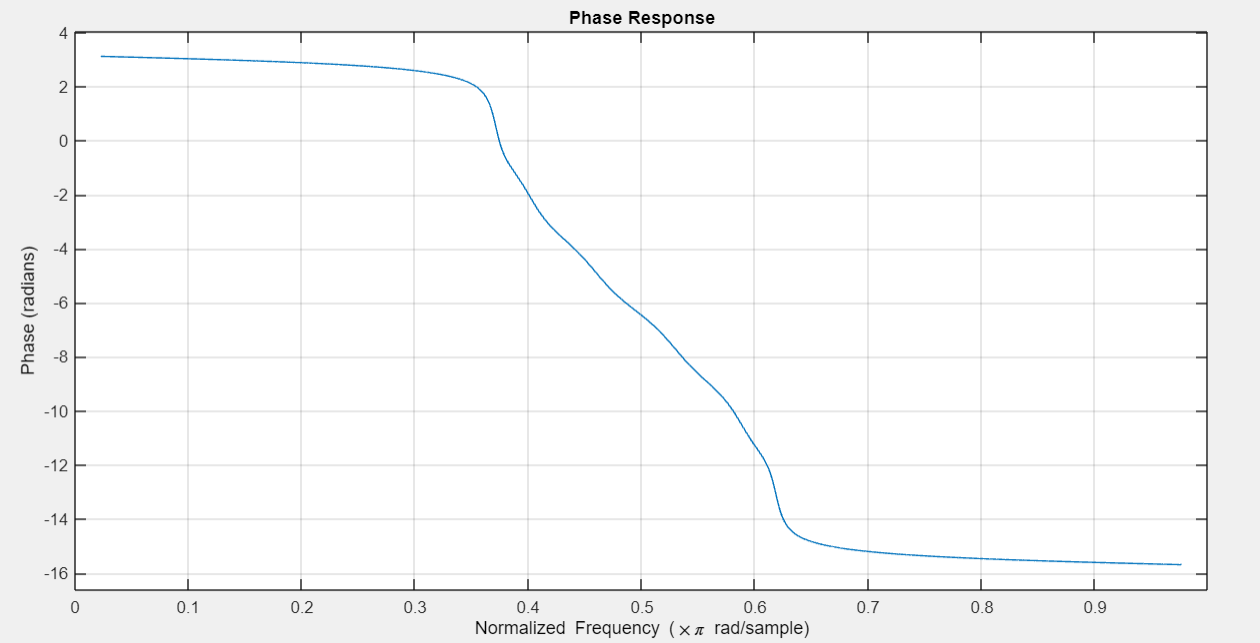
\includegraphics[width =\textwidth, height=10cm]{phase.png}
    \caption{Phase response of the Filter}
\end{figure}

\subsection{Peer Review}

I have reviewed the Chebyschev filter design report of Ojas Karanjkar, Roll No. 210070040. He has used Matlab functions to calculate the parameters and poles required for designing the filter. I have checked the functions and they are correct. Hence, he has calculated all the parameters correctly. He has correctly used transformation from lowpass filter to bandpass filter and used it to find the magnitude and phase response. Hence, his magnitude as well as phase response is also correct.
Thus, I certify that the Chebyschev bandpass filter, designed by Ojas Karanjkar is correct.

\end{document}